\documentclass[12pt,a4paper]{article}
\usepackage{algorithm}
\usepackage{algpseudocode}
\usepackage{listings}
\usepackage{marvosym}
\usepackage{wasysym}
\usepackage{marvosym}
\usepackage{xcolor}
\usepackage{graphicx}
\usepackage{tikz}
\usepackage{tikz-uml}
\usetikzlibrary{positioning,shapes,arrows}
\usetikzlibrary{calc,shapes.multipart,chains,automata,positioning,shapes,arrows,backgrounds,fit}
\usetikzlibrary{matrix,backgrounds}

\author{Sujit Chakrabarti}
\title{Priority Queues and Heaps}
\date{}

\begin{document}
\definecolor{lightblue}{rgb}{0.8,0.93,1.0} % color values Red, Green, Blue
\definecolor{Blue}{rgb}{0,0,1.0} % color values Red, Green, Blue
\definecolor{Red}{rgb}{1,0,0} % color values Red, Green, Blue
\definecolor{Purple}{rgb}{0.5,0,0.5}
\definecolor{Pink}{rgb}{0.7,0,0.2}

\newcommand{\highlight}[1]{{\color{Red}(#1)}}
\newcommand{\comment}[1]{{\color{Blue}#1}}

\lstset{
	language = Java,
	basicstyle = \ttfamily\scriptsize,
	stringstyle = \ttfamily\scriptsize,
	keywordstyle=\color{black}\scriptsize,
	identifierstyle=\color{black}\scriptsize,
	frameround=tttt,
	numbers=none,
	showstringspaces=false
}

\maketitle

\section{Real Life Example}
They represent the natural flow of data or we can say that their structure conveys information
Examples:
\begin{enumerate}
	\item family tree
	\begin{center}
	\resizebox{0.5\textwidth}{!}{%
	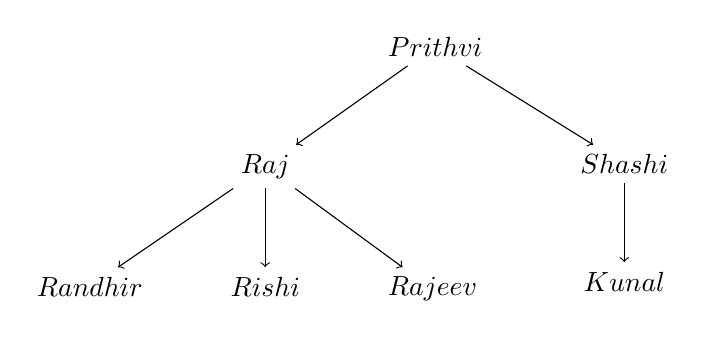
\begin{tikzpicture}
	    \node (A)                      {$Prithvi$};
	    \node (B) [below left  = of A] {$Raj$};
	    \node (C) [below right = of A] {$Shashi$};
	    \node (D) [below left  = of B] {$Randhir$};
	    \node (E) [below       = of B] {$Rishi$};
	    \node (F) [below right = of B] {$Rajeev$};
	    \node (G) [below       = of C]  {$Kunal$};
	    
	    \path[->]
	        (A) edge  (B)
	        (A) edge  (C)
	        (B) edge  (D)
	        (B) edge  (E)
	        (B) edge  (F)
	        (C) edge  (G)
	    ;
	  \end{tikzpicture}
	}
	\end{center}
	
	\item a decision tree
	\includegraphics[width=0.5\textwidth]{images/dt.jpg}

	\item classification of species
	\begin{center}
	\resizebox{0.5\textwidth}{!}{%
	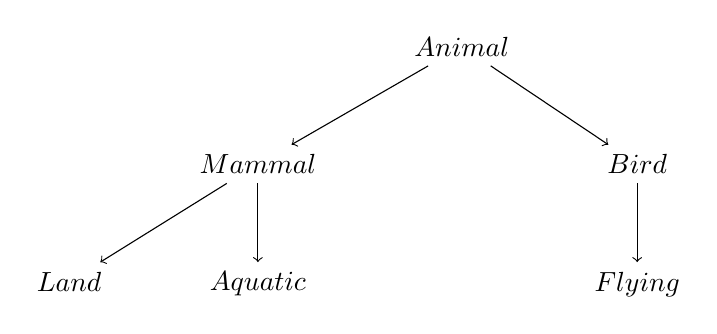
\begin{tikzpicture}
	    \node (A)                      {$Animal$};
	    \node (B) [below left  = of A] {$Mammal$};
	    \node (C) [below right = of A] {$Bird$};
	    \node (D) [below left  = of B] {$Land$};
	    \node (E) [below       = of B] {$Aquatic$};
	    \node (G) [below       = of C]  {$Flying$};
	    
	    \path[->]
	        (A) edge  (B)
	        (A) edge  (C)
	        (B) edge  (D)
	        (B) edge  (E)
	        (C) edge  (G)
	    ;
	  \end{tikzpicture}
	}
	\end{center}


\end{enumerate}

\section{Tree Description} 
\begin{itemize}
	\item root
	\item leaf and internal nodes
	\item parent and child
\end{itemize}

\subsection{Properties}
\begin{itemize}
	\item Unique root
	\item Each node can only have one parent
	\item There can be no cycles in a tree
\end{itemize}


A few demonstrations or examples which do not qualify as a tree.
May be done through an IVQ as well. We will give few structures to the student and ask them to identify which one of them is a tree. 

\section{Binary Tree}
Now we can move on to a particular case of a tree called binary tree. We will learn about it because it’s easier to code. Also, you will learn later that the for basic data structure operations like, insertion deletion, searching etc. binary trees are more efficient than ternary trees.

Define a binary tree

Examples of a binary tree.

Show a visual representation of a binary tree structure

Properties of a Binary Tree:
\begin{enumerate}
\item A parent can have at most two children (one to the left and one to the right)
\end{enumerate}

\section{Traversals}
If we want to visit a particular node, one can not visit it directly like arrays where we use the index of an element and access it. We need to traverse a particular path starting from the root node to reach a node in a tree. Now there can be multiple paths that can be used to access a particular node, let’s see how one path can be more efficient than the other for a particular case. 

Why do we need to traverse along a tree?
How is tree traversal different from a linked list traversal
Why the order in which we traverse a tree is important
This can be explained with the help of a couple of demonstrations where one order is more efficient (in term of runtime) than the other. An example where bfs is more efficient than dfs can be used here. We need not to name the terms, but the example can be used. 
Now that the students know why the order of traversing is important, we can move onto some standard traversal techniques. 

\subsection{Pre Order Traversal}
\subsubsection{Application}
Tree copy, polish notation
\subsubsection{Code}

\subsubsection{Performance}

\subsection{Post order traversal} 
\subsubsection{Application}

\subsubsection{Code}

\subsubsection{Performance}

\subsection{In Order Traversal}
\subsubsection{Application}

\subsubsection{Code}

\subsubsection{Performance}

\subsection{Breadth First Traversal}
\subsubsection{Application}

\subsubsection{Code}

\subsubsection{Performance}

Having learnt various traversal techniques, students need to know that one is not necessarily better than the other. It all depends upon the type of application. 

\subsection{Additional Examples of all traversals (Optional)}

\section{Binary Search Trees (BST)}
\subsection{Introduction, Motivation}
Arrays have an advantage in terms of searching, but linked list are better when it comes to insertion and deletion. Binary trees utilise the advantages of both using something called binary search trees. 

\subsection{Definition of BST}
A visual representation of Binary Search Tree
Binary Search Tree Properties (how it differs from binary trees)
An IVQ where students need to identify a valid BST
Few of the traversal techniques discussed above lead to some interesting results if applied to BST.

Linked list was O(n) when it comes to searching. Let’s see how BST performs here.


\subsection{Search}

\subsubsection{Algorithm}

\subsubsection{Code}

\subsubsection{Efficiency}

\subsubsection{Compare search in a BST to binary search}

\subsection{Insertion}

\subsubsection{Algorithm}

\subsubsection{Code}

\subsubsection{Efficiency}

Linked list are better than arrays when it comes to insertion. BSTs have this advantage also with them. 

\subsection{Deletion}

\subsubsection{Algorithm}

\subsubsection{Code}

\subsubsection{Efficiency}

\subsubsection{Delete an element with no child}

\subsubsection{Delete an element with one child}

\subsubsection{Delete an element with 2 children}

\subsubsection{Efficiency}

\subsubsection{Code}

\subsection{Balanced BSTs}
What is the height of the BST in an average case?
What is the height of the BST in the worse case? (the BST will essentially be a linked list)


\end{document}
